\documentclass[11pt,british,a4paper]{report}
%\pdfobjcompresslevel=0
\usepackage{pythontex}
\usepackage[usenames,dvipsnames]{xcolor}
\usepackage[includeheadfoot,margin=0.8 in]{geometry}
\usepackage{siunitx,physics,cancel,upgreek,varioref,listings,booktabs,pdfpages,ifthen,polynom,todonotes}
%\usepackage{minted}
\usepackage[backend=biber]{biblatex}
\DefineBibliographyStrings{english}{%
      bibliography = {References},
}
\addbibresource{sources.bib}
\usepackage{mathtools,upgreek,bigints}
\usepackage{babel}
\usepackage{graphicx}
\graphicspath{{./}{./e/}}
\usepackage{float}
\usepackage{amsmath}
\usepackage{amssymb,epstopdf}
%\usepackage{fouriernc}
\usepackage[T1]{fontenc}
\usepackage{mathpazo}
% \usepackage{inconsolata}
%\usepackage{eulervm}
%\usepackage{cmbright}
%\usepackage{fontspec}
%\usepackage{unicode-math}
%\setmainfont{Tex Gyre Pagella}
%\setmathfont{Tex Gyre Pagella Math}
\usepackage[scaled]{beramono}
\usepackage{fancyhdr}
\usepackage[utf8]{inputenc}
\usepackage{textcomp}
\usepackage{lastpage}
\usepackage{microtype}
\usepackage[linktoc=all, bookmarks=true, pdfauthor={Anders Johansson},pdftitle={FYS4460 Project 2}]{hyperref}
\usepackage{tikz,pgfplots,pgfplotstable}
\usepgfplotslibrary{colorbrewer}
\usepgfplotslibrary{external}
\tikzexternalize[prefix=data/]
\pgfplotsset{cycle list/Set1}
\pgfplotsset{compat=1.8}
\renewcommand{\CancelColor}{\color{red}}
\let\oldexp=\exp
\renewcommand{\exp}[1]{\mathrm{e}^{#1}}
\renewcommand{\Re}[1]{\mathfrak{Re}\ifthenelse{\equal{#1}{}}{}{\left(#1\right)}}
\renewcommand{\Im}[1]{\mathfrak{Im}\ifthenelse{\equal{#1}{}}{}{\left(#1\right)}}
\renewcommand{\i}{\mathrm{i}}
\newcommand{\tittel}[1]{\title{#1 \vspace{-7ex}}\author{}\date{}\maketitle\thispagestyle{fancy}\pagestyle{fancy}\setcounter{page}{1}}

% \newcommand{\deloppg}[2][]{\subsection*{#2) #1}\addcontentsline{toc}{subsection}{#2)}\refstepcounter{subsection}\label{#2}}
% \newcommand{\oppg}[1]{\section*{Oppgave #1}\addcontentsline{toc}{section}{Oppgave #1}\refstepcounter{section}\label{oppg#1}}

\labelformat{section}{#1}
\labelformat{subsection}{exercise~#1}
\labelformat{subsubsection}{paragraph~#1}
\labelformat{equation}{equation~(#1)}
\labelformat{figure}{figure~#1}
\labelformat{table}{table~#1}

\renewcommand{\footrulewidth}{\headrulewidth}

%\setcounter{secnumdepth}{4}
\renewcommand{\thesection}{Oppgave \arabic{section}}
\renewcommand{\thesubsection}{\alph{subsection})}
\renewcommand{\thesubsubsection}{\arabic{section}\alph{subsection}\roman{subsubsection})}
\setlength{\parindent}{0cm}
\setlength{\parskip}{1em}

\definecolor{bluekeywords}{rgb}{0.13,0.13,1}
\definecolor{greencomments}{rgb}{0,0.5,0}
\definecolor{redstrings}{rgb}{0.9,0,0}
\lstset{rangeprefix=\#/,
    rangesuffix=/\#,
    includerangemarker=false}
\renewcommand{\lstlistingname}{Kodesnutt}
\lstset{showstringspaces=false,
    basicstyle=\ttfamily,
    keywordstyle=\color{bluekeywords},
    commentstyle=\color{greencomments},
    numberstyle=\color{bluekeywords},
    stringstyle=\color{redstrings},
    breaklines=true,
    texcl=true
}
\colorlet{DarkGrey}{white!20!black}
\newcommand{\eqtag}[1]{\refstepcounter{equation}\tag{\theequation}\label{#1}}
\hypersetup{hidelinks=True}

\sisetup{detect-all}
\sisetup{exponent-product = \cdot, output-product = \cdot,per-mode=symbol}
% \sisetup{output-decimal-marker={,}}
\sisetup{round-mode = off, round-precision=3}
\sisetup{number-unit-product = \ }

\allowdisplaybreaks[4]
\fancyhf{}

\rhead{Project 2}
\rfoot{Page~\thepage{} of~\pageref{LastPage}}
\lhead{FYS4460}

%\definecolor{gronn}{rgb}{0.29, 0.33, 0.13}
\definecolor{gronn}{rgb}{0, 0.5, 0}

\newcommand{\husk}[2]{\tikz[baseline,remember picture,inner sep=0pt,outer sep=0pt]{\node[anchor=base] (#1) {\(#2\)};}}
\newcommand{\artanh}[1]{\operatorname{artanh}{\qty(#1)}}
\newcommand{\matrise}[1]{\begin{pmatrix}#1\end{pmatrix}}


\pgfplotstableset{1000 sep={\,},
                      assign column name/.style={/pgfplots/table/column name={\multicolumn{1}{c}{#1}}},
                      every head row/.style={before row=\toprule,after row=\midrule},
                      every last row/.style={after row=\bottomrule},
                      columns/n/.style={column name={\(n^*\)},column type={r}},
                      columns/N/.style={column name={\(N\)},sci},
                      columns/logN/.style={column name={\(\log(N)\)}},
                      columns/logn/.style={column name={\(\log(n^*)\)}}
                      }

\newread\infile

%start
\begin{document}
\title{FYS4460: Project 1}
\author{Anders Johansson}
%\maketitle

\begin{titlepage}
%\includegraphics[width=\textwidth]{fysisk.pdf}
\vspace*{\fill}
\begin{center}
\textsf{
    \Huge \textbf{Project 2}\\\vspace{0.5cm}
    \Large \textbf{FYS4460 - Disordered systems and percolation}\\
    \vspace{8cm}
    Anders Johansson\\
    \today\\
}
\vspace{1.5cm}

\includegraphics{uio.pdf}\\
\vspace*{\fill}
\end{center}
\end{titlepage}
\null
\pagestyle{empty}
\newpage

\pagestyle{fancy}
\setcounter{page}{1}



%   __ _
%  / _` |
% | (_| |
%  \__,_|
%
\subsection{}
I reused the argon script from project 1 but changed the size of the system and the parameter of the lattice command. According to the project description, the lattice spacing should be \(a=\SI{5.72}{\angstrom} = \py{round(5.72/3.405,2)}\sigma\), giving a reduced density (the parameter of the \lstinline{lattice} command) of
\begin{equation}
    \rho^* = \rho\sigma^3 = \frac{4}{\qty(a/\sigma)^3} = \frac{4}{\py{round(5.72/3.405,2)}^3} = \py{round(4/(5.72/3.405)**3,2)}.
\end{equation}

\subsection{}
The system was first thermalised for a certain number of timesteps, determined by looking at the visualisations in the previous exercise. A cylinder was created with the given dimensions, and the atoms inside were selected as a group. The remaining atoms were then given zero velocity for visualisation purposes and excluded from the integration. Visual inspection in Ovito shows that this approach works.

\subsection{}
I considered many options for making spheres with random positions and radii and ended up using the \lstinline{python} command in LAMMPs. This runs a Python function during the execution of the LAMMPs script. The function receives a pointer to a LAMMPs object, which it uses to extract variables and run commands.

The important part of the LAMMPs script is
\lstinputlisting[linerange={snippetstart-snippetend}]{cd/in.script}
The first \lstinline{python} command defines the function \lstinline{make_spheres}, found in the \lstinline{file make_spheres.py}. This function takes \lstinline{1} argument, \lstinline{SELF}, which is a pointer (\lstinline{p}) to the current LAMMPs object. The second \lstinline{python} command runs the Python function. The \lstinline{matrix} group is defined by the Python function as the atoms inside the spheres. The content of \lstinline{make_spheres.py} is the simple function
\lstinputlisting[language=Python]{cd/make_spheres.py}
Periodic boundary conditions are fully enforced by creating all relevant periodic images of each sphere. Unfortunately, the approach of using the \lstinline{python} command inside LAMMPs to run LAMMPS commands does not work well with MPI, so the simulation is run serially.

Visualisation of the result was done by colour coding the atoms according to the magnitude of their velocities, where the lower bound is zero and the upper bound is a very small number. See~\vref{fig:spheres}.
\begin{figure}[H]
    \centering
    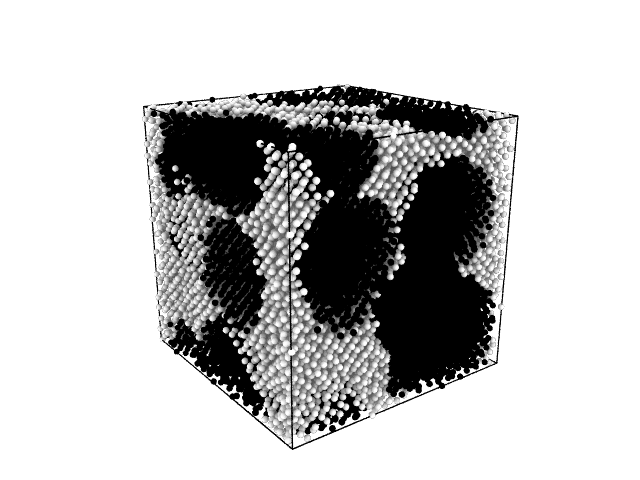
\includegraphics[width=0.5\textwidth]{cd/spheres.png}
    \caption{Visualisation of the randomly placed spheres.}%
    \label{fig:spheres}
\end{figure}

The porosity can be calculated by assuming that the density is the same everywhere. With this assumption, the porosity, which is equal to the volume fraction available for flow, is then equal to the fraction of atoms not inside the rigid matrix. This gives a higher porosity than if the spherical pores were non-overlapping.

\openin\infile=cd/data/porosity.dat
\read\infile to\myporosity
\closein\infile
In LAMMPs, this method of calculating is implemented through a command like \lstinline{variable porosity equal count(moving)/count(all)}, giving the result \(\phi=\num[round-mode=places,round-precision=2]{\myporosity}\).


\subsection{}
See the above exercise.

\subsection{}\label{subsec:e}
Armed with the \lstinline{python} command discovered in the previous exercise, I used the LAMMPs commands
\lstinputlisting[linerange={snippetstart-snippetend}]{e/in.script}
The variable \lstinline{is_moving} is set to \(1\) for all atoms in the group \lstinline{moving} and \(0\) for all atoms in the matrix. The Python function is
\lstinputlisting[language=Python]{e/delete_half_of_moving.py}
Halfway through writing this, I discovered that LAMMPs actually has built-in commands for deleting a certain fraction of the particles in a region, but at that point, there was no turning back. One difficulty of extracting values from \lstinline{lammps} objects is the type of the values returned, which for arrays is a pointer to the underlying C++ structures. This must be converted using \lstinline{numpy.ctypeslib.as_array}.
\begin{pycode}
with open("e/data/beforedeletion.dat","r") as infile1, open("e/data/afterdeletion.dat","r") as infile2:
    before = infile1.read()
    after = infile2.read()
res = r"\(\num{%s}\) and \(\num{%s}\)" % (before, after)
\end{pycode}

The files written by the \lstinline{print} commands in the LAMMPs snippet above contain \py{res}, showing that the number of atoms not in the matrix is indeed halved when the Python function is executed. \Vref{fig:temppores} shows the time evolution of the temperature in the pores.

\begin{figure}[H]
    \centering
    \begin{tikzpicture}
        \begin{axis}[
            thick,
            %axis lines=middle,
            %axis y discontinuity=crunch,
            enlarge x limits=0.05,
            enlarge y limits=0.1,
            width=6in, height=3in,
            xlabel={\(t/\tau\)},
            ylabel={\(T/T_0\)}
            ]
                \addplot+[mark=none] table {e/data/temp.dat};
        \end{axis}
    \end{tikzpicture}
    \caption{Temperature in the pores of the material as a function of time.}%
    \label{fig:temppores}
\end{figure}

\subsection{}
The mean squared displacement of the atoms in the pores was calculated using the \lstinline{compute msd} command in LAMMPs. \Vref{fig:msdpores} shows the result. When \(t\) is large, the mean squared displacement grows linearly with time, while the parabolic trend in the ballistic regime is visible when \(t\ll \tau\).
\begin{figure}[H]
    \centering
    \begin{tikzpicture}
        \begin{axis}[
            thick,
            axis lines=middle,
            %axis y discontinuity=crunch,
            enlarge x limits=0.05,
            enlarge y limits=0.1,
            width=6in, height=3in,
            xlabel={\(t/\tau\)},
            ylabel={\(\ev{r^2(t)}/\sigma^2\)}
            ]
                \addplot+[mark=none] table {e/data/msd.dat};
        \end{axis}
    \end{tikzpicture}
    \caption{Mean squared displacement in the pores of the material as a function of time. As expected, the result is linear when \(t\) is large and approximately parabolic when \(t\) is small.}%
    \label{fig:msdpores}
\end{figure}

\subsection{}
Darcy's law is
\begin{equation}
    U = \frac{k}{\mu}\qty(\nabla P - \rho g),
\end{equation}
where \(U\) is the volume flux density, \(k\) is the permeability, \(\nabla P\) is the gradient of the external pressure (non-existent in this project), \(\rho\) is the mass density and \(g\) is the net acceleration due to externally applied forces. The applied force points in the \(x\)-direction, and \(F_x\) is the force applied to each atom. Newton's second law for a system of \(N\) atoms in a volume \(V\) with the force \(F_x\) applied to each is thus
\begin{equation}
    NF_x = Nmg.
\end{equation}
This can be divided by the volume, giving
\begin{equation}
    \frac{Nm}{V}g = \rho g = \frac{N}{V}F_x = nF_x,
\end{equation}
where \(n\) is the number density.

\subsection{}
(I choose to redo the analytical solution for the velocity field with an applied force instead of an applied pressure gradient for my own reference and understanding.)

I here assume that we are dealing with a Newtonian fluid, defined as a fluid in which the viscous forces due to a difference in the \(\hat{e}_i\) component of the velocity create a force in the \(\hat{e}_i\)-direction on a surface with normal \(\hat{e}_j\) that is proportional to the derivative of the velocity when going in the \(\hat{e}_j\)-direction,
\begin{equation}
    \sigma_{ij}\ \qty(\equiv \frac{F_i}{A_j}) = \mu \pdv{v_i}{x_j}.\label{eq:newtfluid}
\end{equation}
The quantity \(\mu\) is the viscosity, while \(\sigma_{ij}\) is the stress tensor. In a cylindrical pore orientated in the \(x\)-direction with radius \(a\), the velocity field should be independent of the angle with the \(x\)-axis and only depend on the distance to the centre of the cylinder.

A small volume element in cylindrical coordinates has volume \(r\dd{\phi}\dd{r}\dd{x}\). It is acted upon by two forces in the \(x\)-direction:
\begin{itemize}
    \item The externally applied force. With the number density \(n\), the number of particles in the volume element is \(nr\dd{\phi}\dd{r}\dd{x}\), giving a total force
        \begin{equation}
            F_{\text{ext}} = nF_xr\dd{\phi}\dd{r}\dd{x}.
        \end{equation}
    \item
        Viscous forces due to the radial dependence of the velocity. According to~\vref{eq:newtfluid}, the force on the ``outer'' surface of the volume element, whose normal is directed radially outwards, is
        \begin{equation}
            F_{\text{outer}} = \mu \eval{\pdv{v_x}{r}}_{r=r+\dd{r}}\overbrace{\qty(r+\dd{r})\dd{\phi}\dd{x}}^{A_r},
        \end{equation}
        while the force on the ``inner'' surface, whose normal is directed radially inwards, is
        \begin{equation}
            F_{\text{inner}} = -\mu \eval{\pdv{v_x}{r}}_{r=r}r\dd{\phi}\dd{x}.
        \end{equation}
        The minus sign is due to the normal of the surface being \(-\hat{e}_r\). Without the minus, it would be the force from ``our'' volume element, \(r\in\qty[r,r+\dd{r}]\), on the volume element with \(r\in\qty[r-\dd{r},r]\). Newton's third law says that the required correction is a minus sign. Due to the assumption of rotational invariance there are no other viscous forces.
\end{itemize}
In equilibrium, the sum of these forces must be zero from Newton's first law. This gives
\begin{equation}
    \mu\qty(\eval{\pdv{v_x}{r}}_{r+\dd{r}}\qty(r+\dd{r})-\eval{\pdv{v_x}{r}}_{r}r)\dd{\phi}\dd{x} + nF_xr\dd{\phi}\dd{r}\dd{x} = 0.
\end{equation}
I now divide by \(\dd{\phi}\dd{r}\dd{x}\), recognize the resulting first term as the derivative of \(r\pdv*{v_x}{r}\) and move some terms, resulting in the differential equation
\begin{equation}
    \pdv{r}(r\pdv{v_x}{r}) = -\frac{nF_x}{\mu}r.
\end{equation}
Everything except \(r\) is constant on the right-hand side, so this equation can be integrated directly to yield the \(x\) component of the velocity as a function of \(r\),
\begin{equation}
    r\pdv{v_x}{r} = -\frac{1}{2}\frac{nF_x}{\mu}r^2 + C
    \implies \pdv{v_x}{r} = -\frac{nF_x}{2\mu}r + C/r
    \implies v_x(r) = -\frac{nF_x}{4\mu}r^2 + C\ln r + D.
\end{equation}
The velocity should not be problematic when \(r=0\), i.e.\ in the centre of the cylinder, so \(C\) must be zero. The second integration constant, \(D\), is determined by the choice of boundary conditions. A reasonable assumption for a solid-liquid interface is zero velocity at the boundary, which in this case is \(r=a\). This implies \(D=nF_xa^2/4\mu\), giving the velocity profile
\begin{equation}
    v_x(r) = \frac{nF_x}{4\mu}\qty(a^2-r^2).\label{eq:velprofile}
\end{equation}
Comparing this to the result from the lectures shows that \(\Delta P/L = \nabla P\) is replaced by \(-nF_x\) when a force is applied instead of a pressure gradient.

Darcy's law contains the volume flux density, i.e.\ the amount of volume passing through a cross-section per time per area, \(U=\dd{V}/A\dd{t}\). The infinitesimal volume must be
\begin{equation}
\dd{V}=A\dd{x}=A\bar{v}_x\dd{t},
\end{equation}
where \(A\) is the area of the cross-section and \(\bar{v}_x\) is the average velocity in the \(x\)-direction. Consequently \(U=\bar{v}_x\). The mean velocity can be calculated as
\begin{alignat}{2}
    U &= \bar{v}_x = \frac{1}{A}\int v_x \dd{A} = \frac{1}{\pi a^2}\int_0^a v(r)\cdot 2\pi r\dd{r}\\
    &= \frac{nF_x}{2\mu a^2}\int_0^a \qty(a^2-r^2)r\dd{r}
    = \frac{nF_x}{2\mu a^2}\qty(\tfrac{1}{2}a^4-\tfrac{1}{4}a^4)
    = \frac{nF_xa^2}{8\mu} = \frac{k}{\mu} nF_x,\label{eq:meanvel}
\end{alignat}
which is just Darcy's law for an externally applied force, where \(k=a^2/8\).

The viscosity can now be determined numerically by running simulations and comparing the resulting velocity profile (at equilibrium) to~\vref{eq:velprofile}, while the permeability for an arbitrary geometry can be calculated from~\vref{eq:meanvel} with the viscosity found from a cylindrical pore.

I here choose to study the fluid flow of argon with half the density, using the method developed in~\vref{subsec:e} to delete half of the moving atoms. The setup is otherwise as in the first exercises with a cylindrical pore.

The velocity of the centre of mass of a group can be calculated by LAMMPs. This is equal to the mean velocity of the atoms in the group. \Vref{fig:cylindervxcm} shows the time evolution, while~\vref{fig:cylindervx} shows the radial distribution after the system has reached equilibrium.

\begin{pycode}
with open("h/data/viscosity.dat","r") as infile:
    mu = float(infile.read())
mutxt = r"\num{%.2g}" % mu
\end{pycode}

From~\vref{eq:velprofile}, the radial distribution should be a linear function of \(nF_x\qty(a^2-r^2)/4\) with slope \(1/\mu\). I use this relation to approximate the viscosity, resulting in
\begin{equation}
    \mu \approx \py{mutxt}\ \varepsilon\tau/\sigma^3. \label{eq:viscosity}
\end{equation}
According to the internet, this is only \(\SI{50}{\percent}\) too large.
\Vref{fig:cylindervx} shows the quality of the approximation. The number density is approximated by \(2/b^3\), as there are initially \(4\) atoms per face-centred cubic unit cell with volume \(b^3\).
\begin{figure}[H]
    \centering
    \begin{tikzpicture}
        \begin{axis}[
            thick,
            %axis lines=middle,
            %axis y discontinuity=crunch,
            enlarge x limits=0.05,
            enlarge y limits=0.1,
            width=6in, height=3in,
            xlabel={\(t/\tau\)},
            ylabel={\(\bar{v}_x\tau/\sigma\)}
            ]
                \addplot+[mark=none] table {h/data/vxcm.dat};
        \end{axis}
    \end{tikzpicture}
    \caption{Mean velocity in the \(x\)-direction of atoms in the cylinder as a function of time. The system appears to reach equilibrium after approximately \(100\tau\), or \(\num{20000}\) timesteps.}%
    \label{fig:cylindervxcm}
\end{figure}
\begin{figure}[H]
    \centering
    \begin{tikzpicture}
        \begin{axis}[
            legend style={draw=none},
            legend cell align=left,
            thick,
            axis lines=middle,
            xlabel style={anchor=north west},
            ylabel style={anchor=east},
            %axis y discontinuity=crunch,
            enlarge x limits=0.05,
            enlarge y limits=0.1,
            width=6in, height=3in,
            xlabel={\(r/\sigma\)},
            ylabel={\(\bar{v}_x\tau/\sigma\)}
            ]
                \addplot+[mark=none] table {h/data/v.dat};
                \addlegendentry{Simulation result};
                \addplot+[mark=none] table {h/data/vapprox.dat};
                \addlegendentry{Approximation, \ref{eq:velprofile}};
        \end{axis}
    \end{tikzpicture}
    \caption{Radial distribution of the mean velocity in the \(x\)-direction of atoms in the cylinder in equilibrium. The result is an average over all dumped timesteps after the one determined by looking at ~\vref{fig:cylindervxcm}.}%
    \label{fig:cylindervx}
\end{figure}
A few comments on the implementation:
\begin{itemize}
    \item The radial distribution is made by finding all the \(x\)-components of the velocities of the atoms, binning them by the atom's distance to the centre of the cylinder, and taking the average velocity in each bin. Additionally, the result is averaged over time for all saved data sets with the system in equilibrium.
    \item Initially the radial bins had linearly spaced radii. This causes the number of atoms per bin to increase linearly with the bin number, which means that very few atoms are in the inner bins. As a result, the statistics were not very good. My solution was to distribute the radial bin edges as the square root of linearly spaced values from \(0\) to \(a^2\), resulting in an approximately uniform distribution of particles.
    \item The radial bin averaging was done by \lstinline{scipy.stats.binned_statistics}. Unfortunately, Scipy is not easily available inside the Ovitos interpreter, so the dump files had to be read manually. Fortunately, the LAMMPs dump format is very suitable for programmed reading.
\end{itemize}

\subsection{}
The permeability as a function of porosity can be found by using~\vref{eq:meanvel} with the viscosity from~\vref{eq:viscosity} for a set of porosities. I here choose to vary the porosity simply by varying the number of spheres in the matrix.

A rough theoretical model for the permeability is\cite{feder_flow_1984}
\begin{equation}
    k = \frac{a^2}{45}\frac{\phi^3}{\qty(1-\phi)^2},\label{eq:modelpermeability}
\end{equation}
which is compared with the simulation results in~\vref{fig:permeability}. The fit is not very good, apart from a similar trend.

Since each simulation takes a non-trivial amount of time to run, I avoid redoing simulations with the following \lstinline{make} rule.
\lstinputlisting[linerange={snippetstart-snippetend}]{{i/Makefile}}
A \lstinline{Pool} object from \lstinline{multiprocessing} is used to call a Python analysis function for each number of spheres in parallel. This function issues a \lstinline{make} command, reads the resulting log file and calculates the permeability from~\vref{eq:meanvel}. The result is shown in~\vref{fig:permeability}.

One way to improve the fit between the simulation results and the theoretical model might be upscaling the entire system, as the theoretical model holds for the continuum behaviour of fluids. This requires that all distances between rigid spheres must be larger than a certain length, probably on the order of \(\SI{1}{\nano\m}\). A total system size of approximately \(\SI{10}{\nano\m}\) is most likely too small to achieve continuum behaviour.
\begin{figure}[H]
    \centering
    \begin{tikzpicture}
        \begin{axis}[
            legend style={draw=none,at={(0.4,0.8)}},
            legend cell align=left,
            thick,
            %axis lines=middle,
            xlabel style={anchor=north west},
            ylabel style={anchor=east},
            %axis y discontinuity=crunch,
            enlarge x limits=0.05,
            enlarge y limits=0.1,
            width=6in, height=3in,
            xlabel={\(\phi\)},
            ylabel={\(k/\sigma^2\)},
            xtick distance=0.05,
            ]
                \addplot+[mark=none] table {i/data/permeability.dat};
                \addlegendentry{Simulation result};
                \addplot+[mark=none] table {i/data/model.dat};
                \addlegendentry{Theoretical model};
        \end{axis}
    \end{tikzpicture}
    \caption{Permeability as a function of porosity in a system with spheres making up the matrix. Comparison with the theoretical model in~\vref{eq:modelpermeability} shows that the fit is not particularly good, but at least the trend is somewhat similar.}%
    \label{fig:permeability}
\end{figure}


































\nocite{*}
\printbibliography{}
\addcontentsline{toc}{chapter}{\bibname}
\end{document}
